\section{Introduction}

Autonomous vehicles are considered to be one of the most challenging
types of reactive systems currently under development~\cite{AlurMT16,
  WongpiromsarnKF11, RamanDSMS15}. They need to interact reliably with
a highly reactive environment and crashes cannot be tolerated.  Life
critical decisions have to be made instantaneously and need to be
executed at the right point in time.

The development of autonomous vehicles and other cyberphysical systems
is supported by a wide spectrum of
programming and modelling methodologies, 
including synchronous programming languages like Lustre and Esterelle,
hardware-oriented versions of imperative programming languages like
SystemC, and visual languages like MSCs and Stateflow-charts.
The question which programming paradigm is best-suited to write
easy-to-understand, bug-free code is still largely unresolved.

In the development of other forms of critical software, outside the
embedded domain, developers increasingly turn to functional
programming (cf.~\cite{financialsoftware}).  The strong type system in functional
languages~\cite{cardelli1996type} largely eliminates runtime errors.
Higher-order functions like \texttt{map} often eliminate the need for
explicit index counters, and, hence, the risk of ``index out of
bounds'' errors.  Functional purity reduces the possibility of
malformed state that can cause unexpected behavior.

While mathematical models of embedded and cyberphysical systems often
rely on functional notions such as stream-processing
functions~\cite{DBLP:series/mcs/BroyS01,DBLP:conf/csdm/Broy12}, the
application of functional programming in the practical development of
such systems has, so far, been limited. One of the most advanced
programming language in this direction is Ivory, which was used in the
development autonomous vehicles~\cite{pike2014}.  Ivory is a
restricted version of the C programming language, embedded in Haskell.
It provides access to the low level operations necessary for embedded
system programming, but still enforces good programming practice, such
as disallowing pointer arithmetic, with a rich type system.

Ivory does not, however, deal with the integration of 
continuous and discrete time, which is fundamental for the
development of a cyberphysical system. For example,
In a car, continuous signals such as the velocity, acceleration, etc.
mix with the discrete steps of the digital controller.

In this paper, we investigate the use of functional programming
in a domain where the interaction between continous and discrete signals
is of fundamental importance. We build a vehicle controller capable
of both autonomous vehicle control and multi-vehicle communication,
such as the coordination in platooning situations.

Our approach is based on Functional Reactive Programming
(FRP)~\cite{hudak2003arrows,hudak2000haskell}.
The fundamental idea of FRP is to extend the classic building blocks 
of functional programming (\eg monads, arrows,
applicatives)
with the abstraction of a \emph{signal} to
describe time-varying values. FRP programs can be exceptionally
efficient.  For example, a network controller recently implemented as
an FRP program on a multicore processor outperforms any other such
controller existing today~\cite{Voellmy:2012:SSD:2377677.2377735}.

We have built a library, \ourLib, to use FRP to control a vehicle inside a simulation.
The library interfaces Haskell FRP programs to TORCS, The Open Racing Car Simulator, an open-source vehicle simulator~\cite{torcs}.
TORCS has been used in the Simulated Car Racing Championship competition~\cite{SCRC}.
Through \ourLib, the Haskell program has access to the sensors and actuators of the car, as well
as the communication channels between different vehicles.
Such a simulator is a  critical component of modern autonomous vehicle research, especially towards the goal of safe platooning algorithms~\cite{?}.

We report on experience with a case study, in which we implement a controller for a car on an empty race trace. Our controller successfully navigates, with considerable speed and finesse (see Fig.~\ref{fig:race}). Furthermore, the case study illustrates that the functional approach indeed leads to elegant, easily
understandable, and safe code.

\begin{figure}[t]
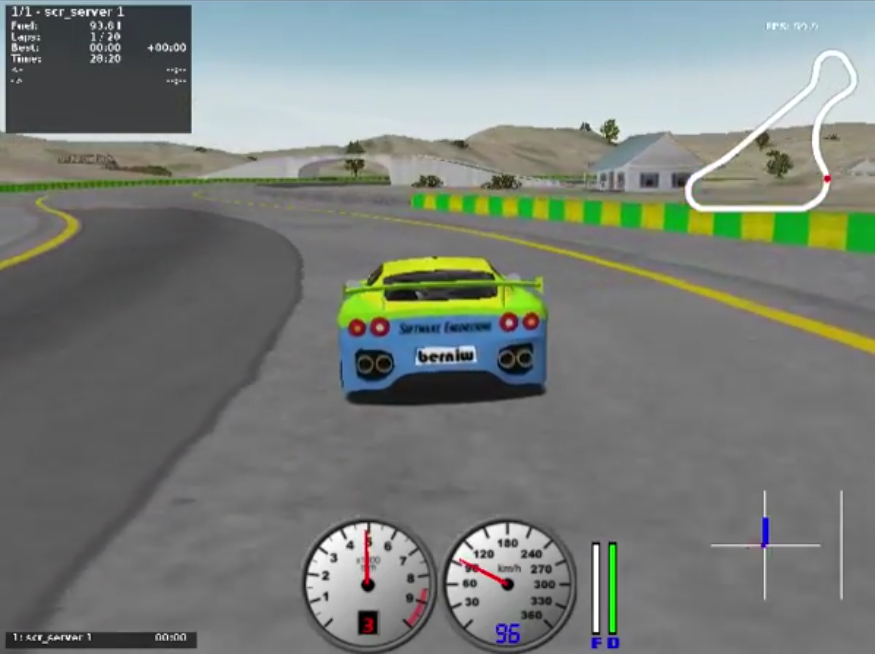
\includegraphics[width=0.45\textwidth]{figs/racing.png}
\caption{A screenshot of Haskell controlling the autonomous vehicle in the TORCS simulator}
\label{fig:race}
\end{figure}
